\subsection{Transporte radial y las leyes de Fick}

A partir de ahora trabajaremos con los electrones en el plasma y dejaremos de lado los sub\'indices. De momento, bajo un transporte cl\'asico donde el campo magn\'etico es homogeneo asumimos que las leyes de Fick se sostienen tal que $q_j = -\chi_{jk}\partial_k T$ y $\Gamma_j = -D_{jk}\partial_k n$, m\'as adelante justificaremos esto. La configuraci\'on del modelo es como se ve en la figura \label{fig:pgeom}. 

\begin{figure}[htb!]\label{fig:pgeom}
		\centering
		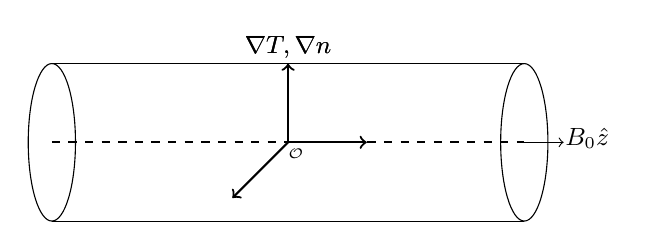
\begin{tikzpicture}[scale=1]
			% Cylinder axis from left to right
			(0,0) ellipse (0.3 and 1) % left cap
			(6,0) ellipse (0.3 and 1); % right cap (hidden)
			% Body
			(0,1) -- (6,1) arc (90:-90:1 and 0.3) -- (0,-1) arc (-90:90:1 and 0.3);
			% Front and back ellipses
			\draw (0,0) ellipse (0.3 and 1);
			\draw (6,0) ellipse (0.3 and 1);
			\foreach \angle in {0,90, 225}{
				\draw[->,thick] (3,0) -- ++(\angle:1);
			}\foreach \angle in {0,90}{
				\node at (3,1.2) {\small{$\nabla T, \nabla n$}} ++(\angle:1);
			}
			\node at (3.1,-0.15) {\tiny{$\mathcal{O}$}};
			% Cylinder outline
			\draw (0,1) -- (6,1);
			\draw (0,-1) -- (6,-1);
			\draw[dashed, thick] (0.0,0.0) -- (6.0,0.0);
			\draw[->] (6.0,0.0) -- (6.5,0.0);
			\node at (6.8,0.05) {\small{$B_0\hat{z}$}};
		\end{tikzpicture}
		\caption{Plasma Cil\'indrico con campo uniforme y transporte radial de part\'iculas y energ\'ia}
	\end{figure}

Se pueden ver que finalmente las relaciones de transporte radial, o flujo de part\'iculas y energ\'ia se pueden escribir como

  \begin{eqnarray}
    \Gamma_n &=& -A\left<\textbf{D}\cdot\nabla n\right>_{\partial V} \label{eq:partflux}\\
    \Gamma_E &=& -A\left<\pmb{\chi}\cdot\nabla T\right>_{\partial V} + \frac{3}{2}A\left<T\pmb{\Gamma}\right>_{\partial V}\label{eq:energyflux}
    \end{eqnarray}
    
  Las cantidades $\chi$ y $D$ deben ser estudiadas m\'as a fondo antes de asumir que son simplemente coeficientes, ya que podr\'an depender de la densidad $n$ y la temperatura $T$.
